\section{Experiments}
In this part we compare MLE with GP and Naive method. 
\subsection{Data}
\subsubsection{Synthetic}
Synthetic datasets are created as follows. Firs using msms prgram, we created a population for $F$ founding haplotypes. Then a population of n homozygote diploid individuals are randomly created as initial population for each simulation. Given initial population, we used simuPop to perform forward simulation by randomly choosing the site under selection. Allele frequency of the populations at generations 10,20,30,40,50 are recorded, i.e. $\Tc=\{10,20,30,40,50\}$
\subsubsection{Real}

\subsection{Results}
\subsubsection{Detecting Selection}
\begin{figure}[H]
  \centering
    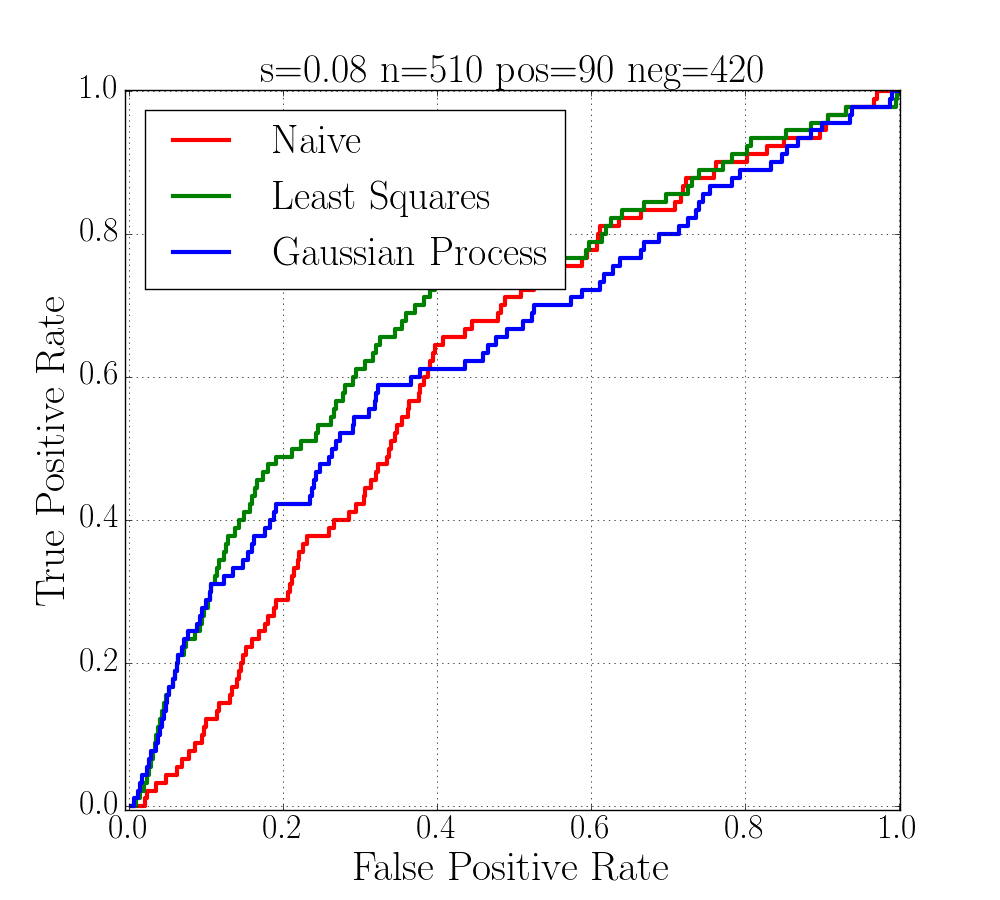
\includegraphics[width=\textwidth]{roc008}
  \caption{Rank}
  \label{fig:Fig3}
\end{figure}

\begin{figure}[H]
  \centering
    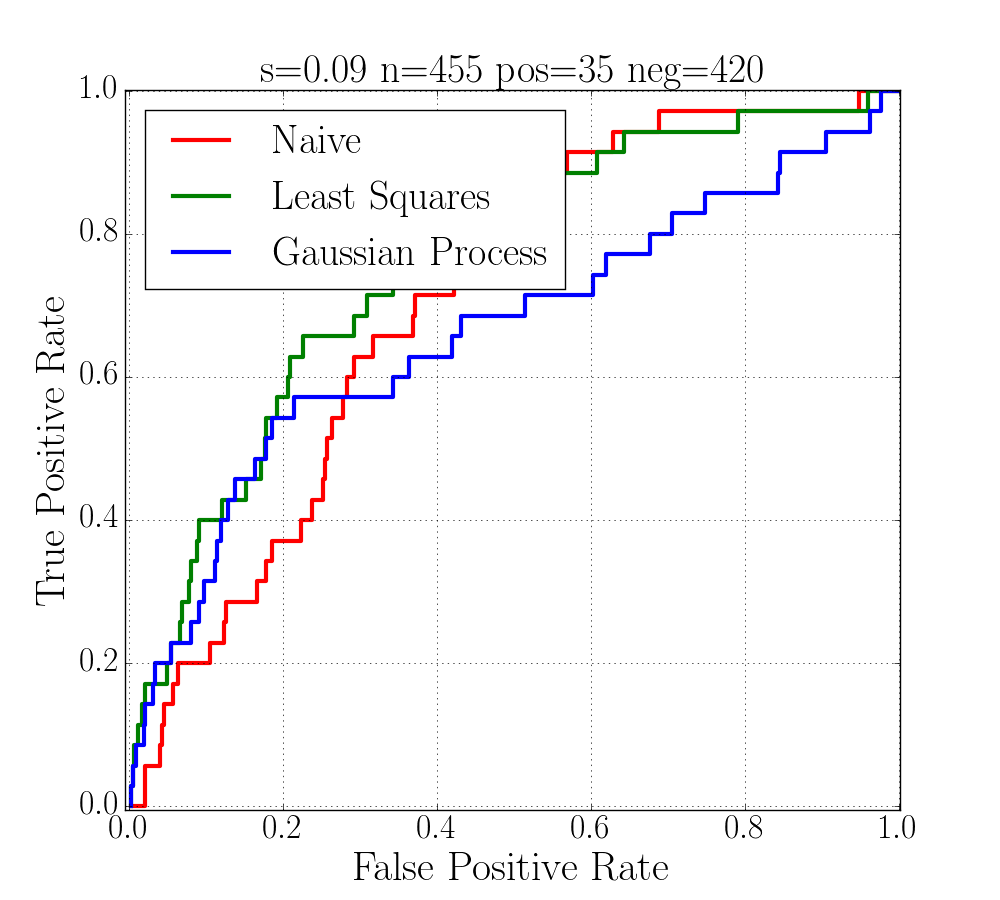
\includegraphics[width=\textwidth]{roc009}
  \caption{Rank}
  \label{fig:Fig3}
\end{figure}

\begin{figure}[H]
  \centering
    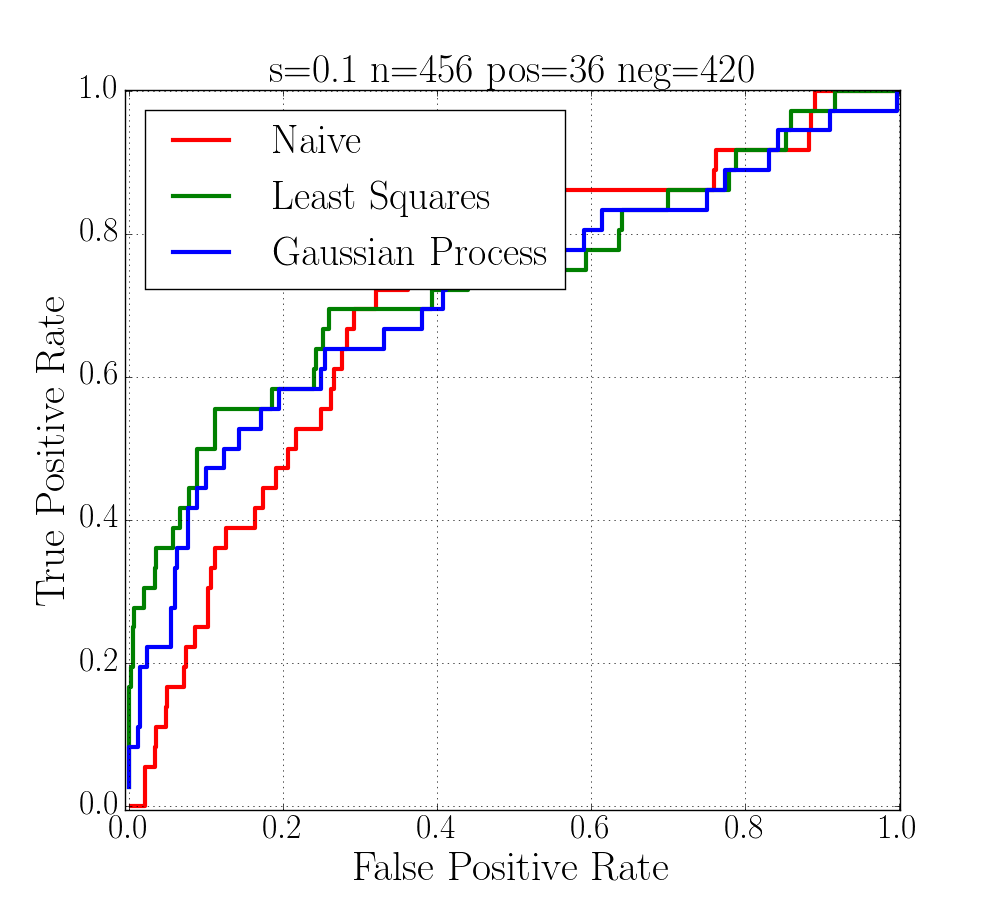
\includegraphics[width=\textwidth]{roc01}
  \caption{Rank}
  \label{fig:Fig3}
\end{figure}


\subsubsection{Finding Site Under Selection}
\paragraph{Distance}
\begin{figure}[H]
  \centering
    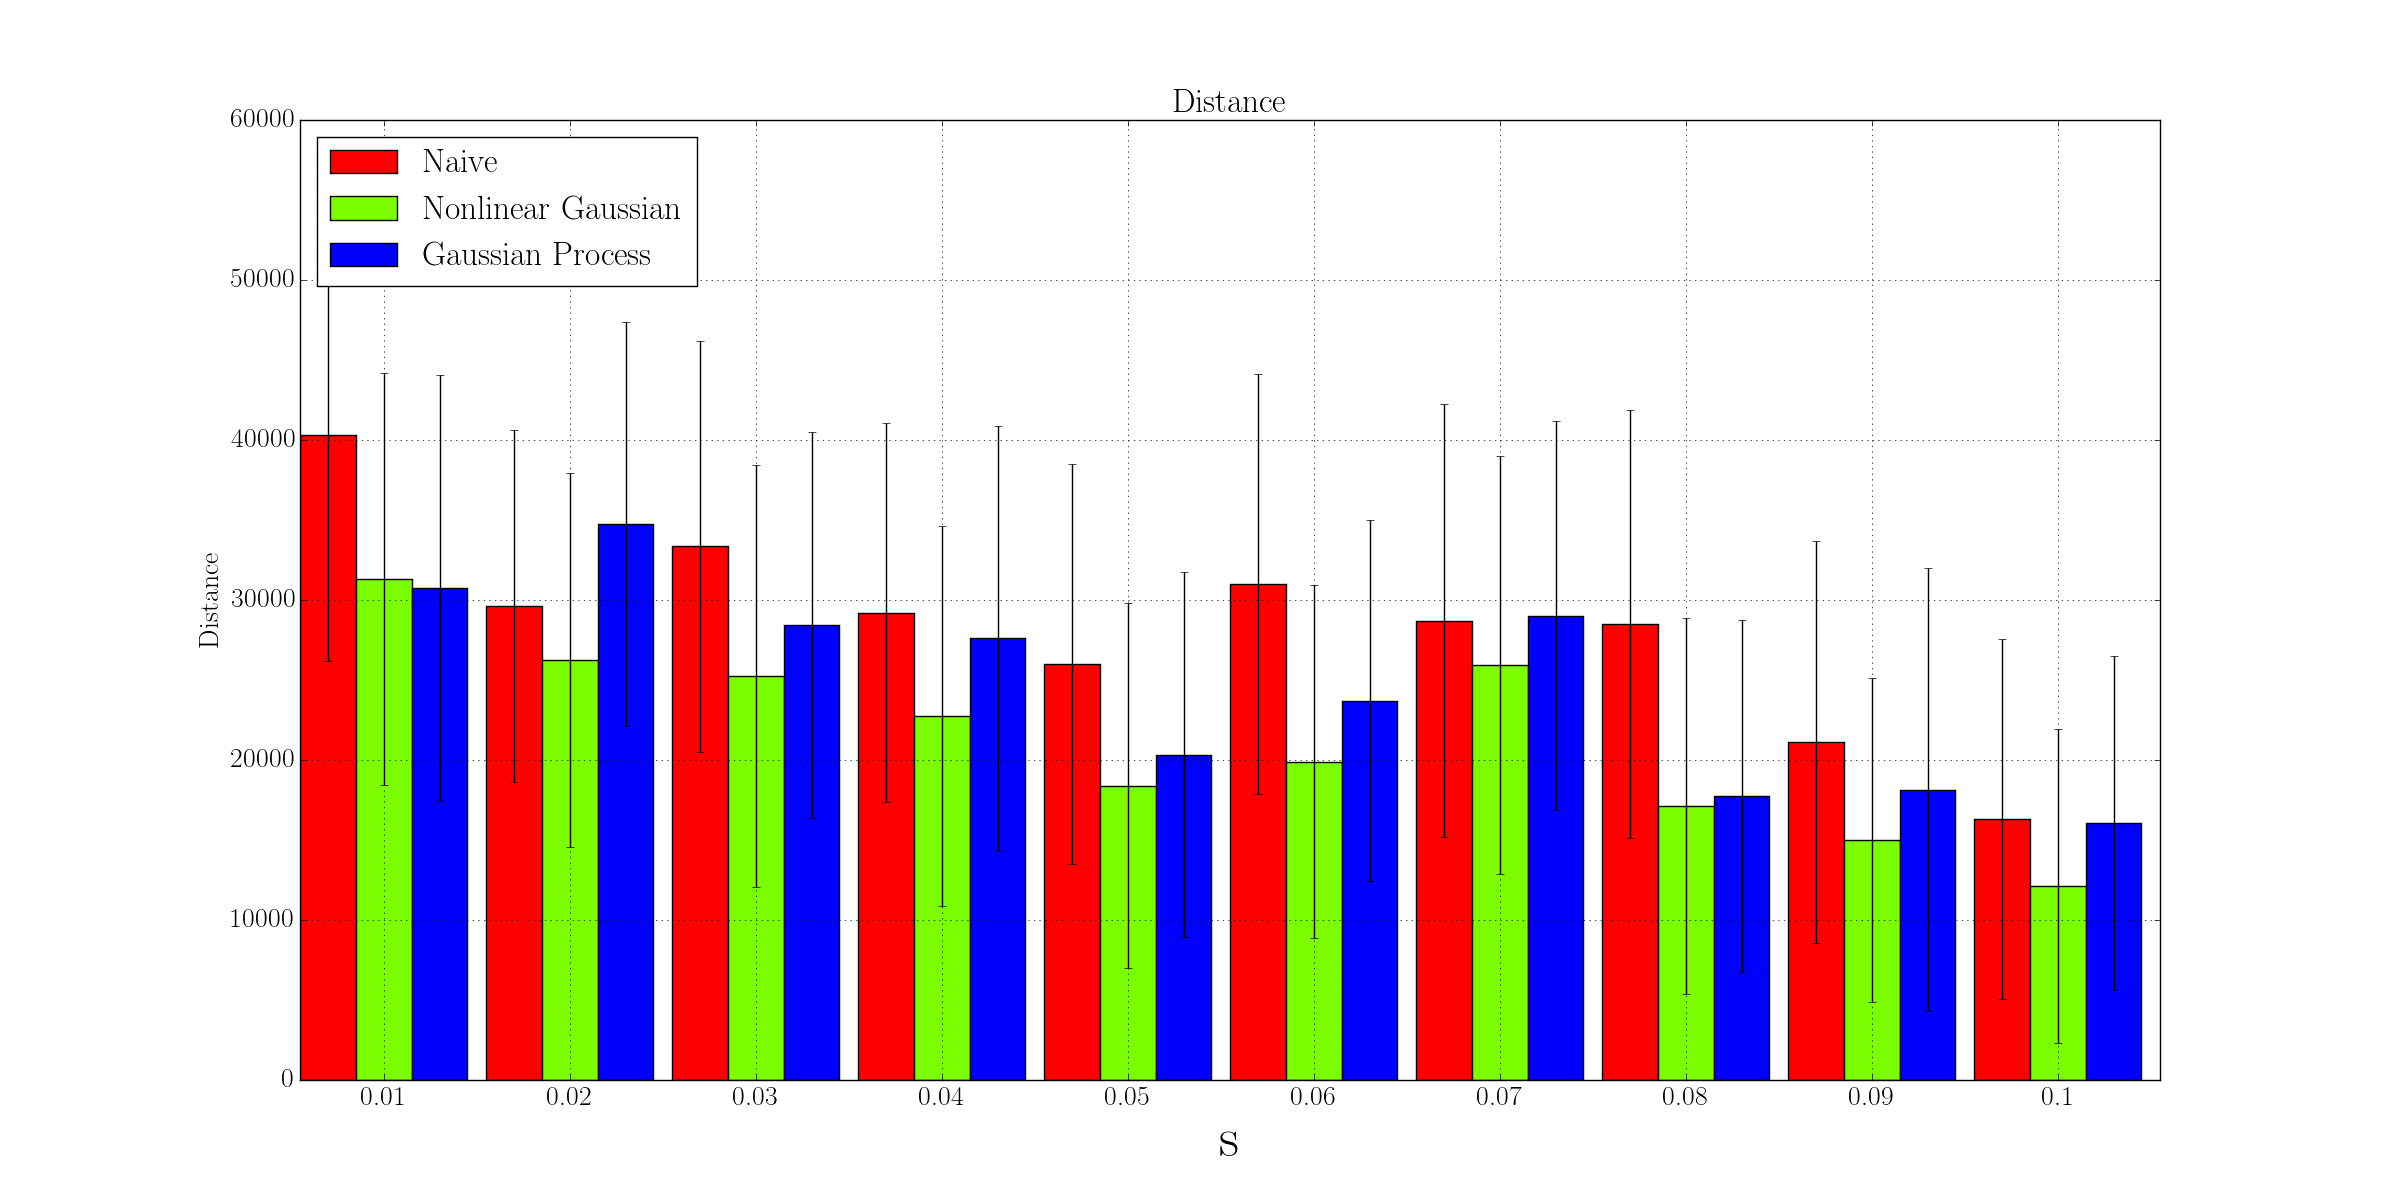
\includegraphics[width=\textwidth]{dist}
  \caption{Average distance to predicted site to the true site that is under selection.}
  \label{fig:Fig1}
\end{figure}

\paragraph{Rank}
\begin{figure}[H]
  \centering
    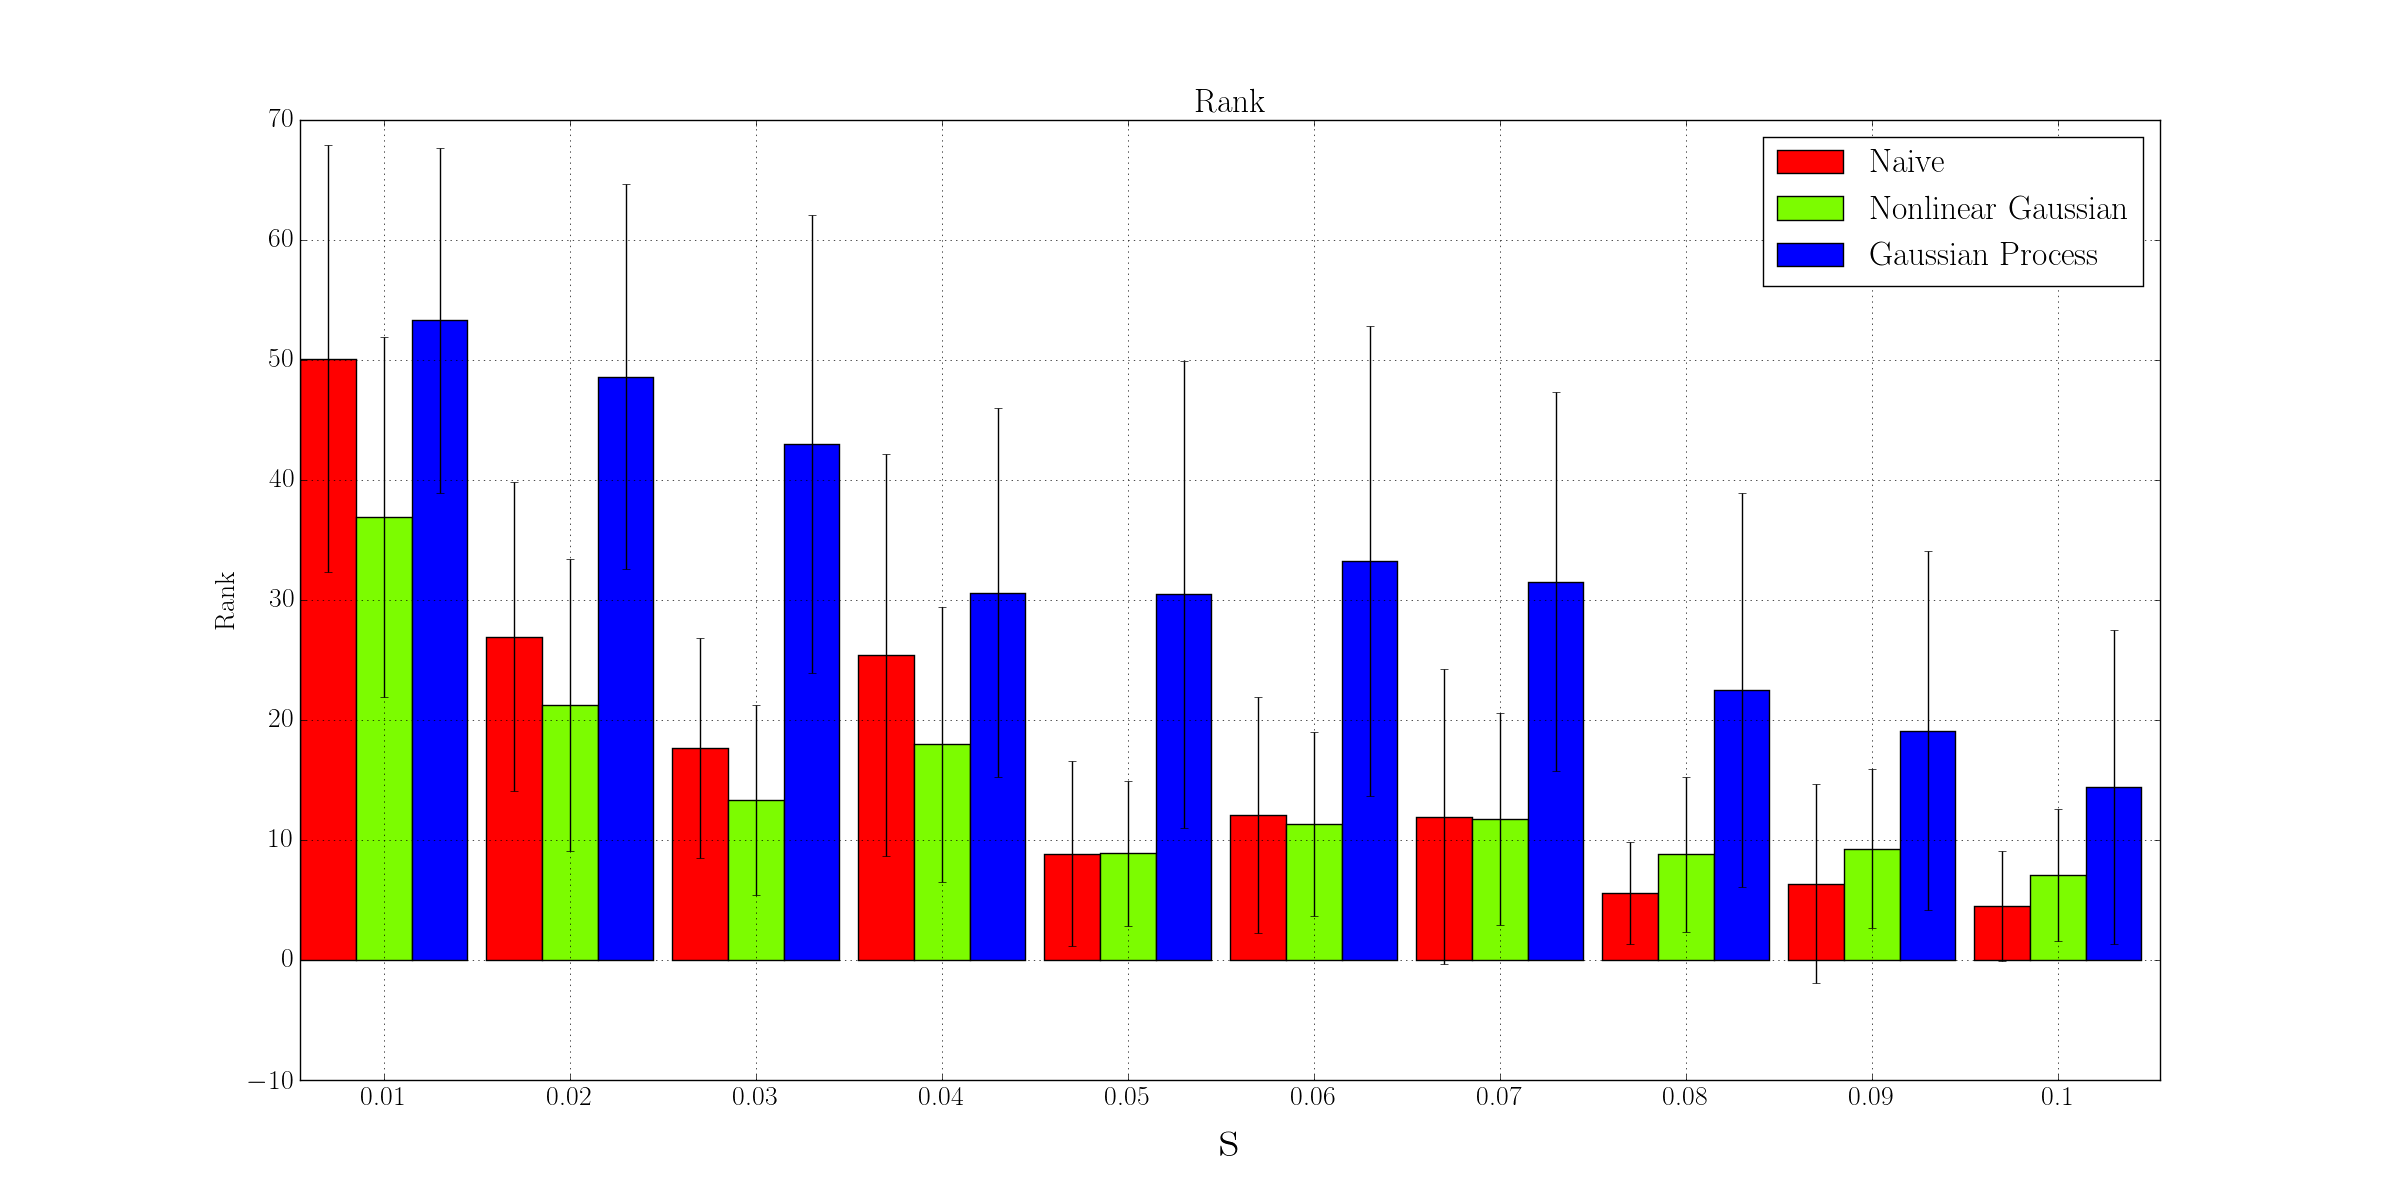
\includegraphics[width=\textwidth]{rank}
  \caption{Rank}
  \label{fig:Fig3}
\end{figure}

\paragraph{Mean Reciprocal Rank(MRR)}
\begin{figure}[H]
  \centering
    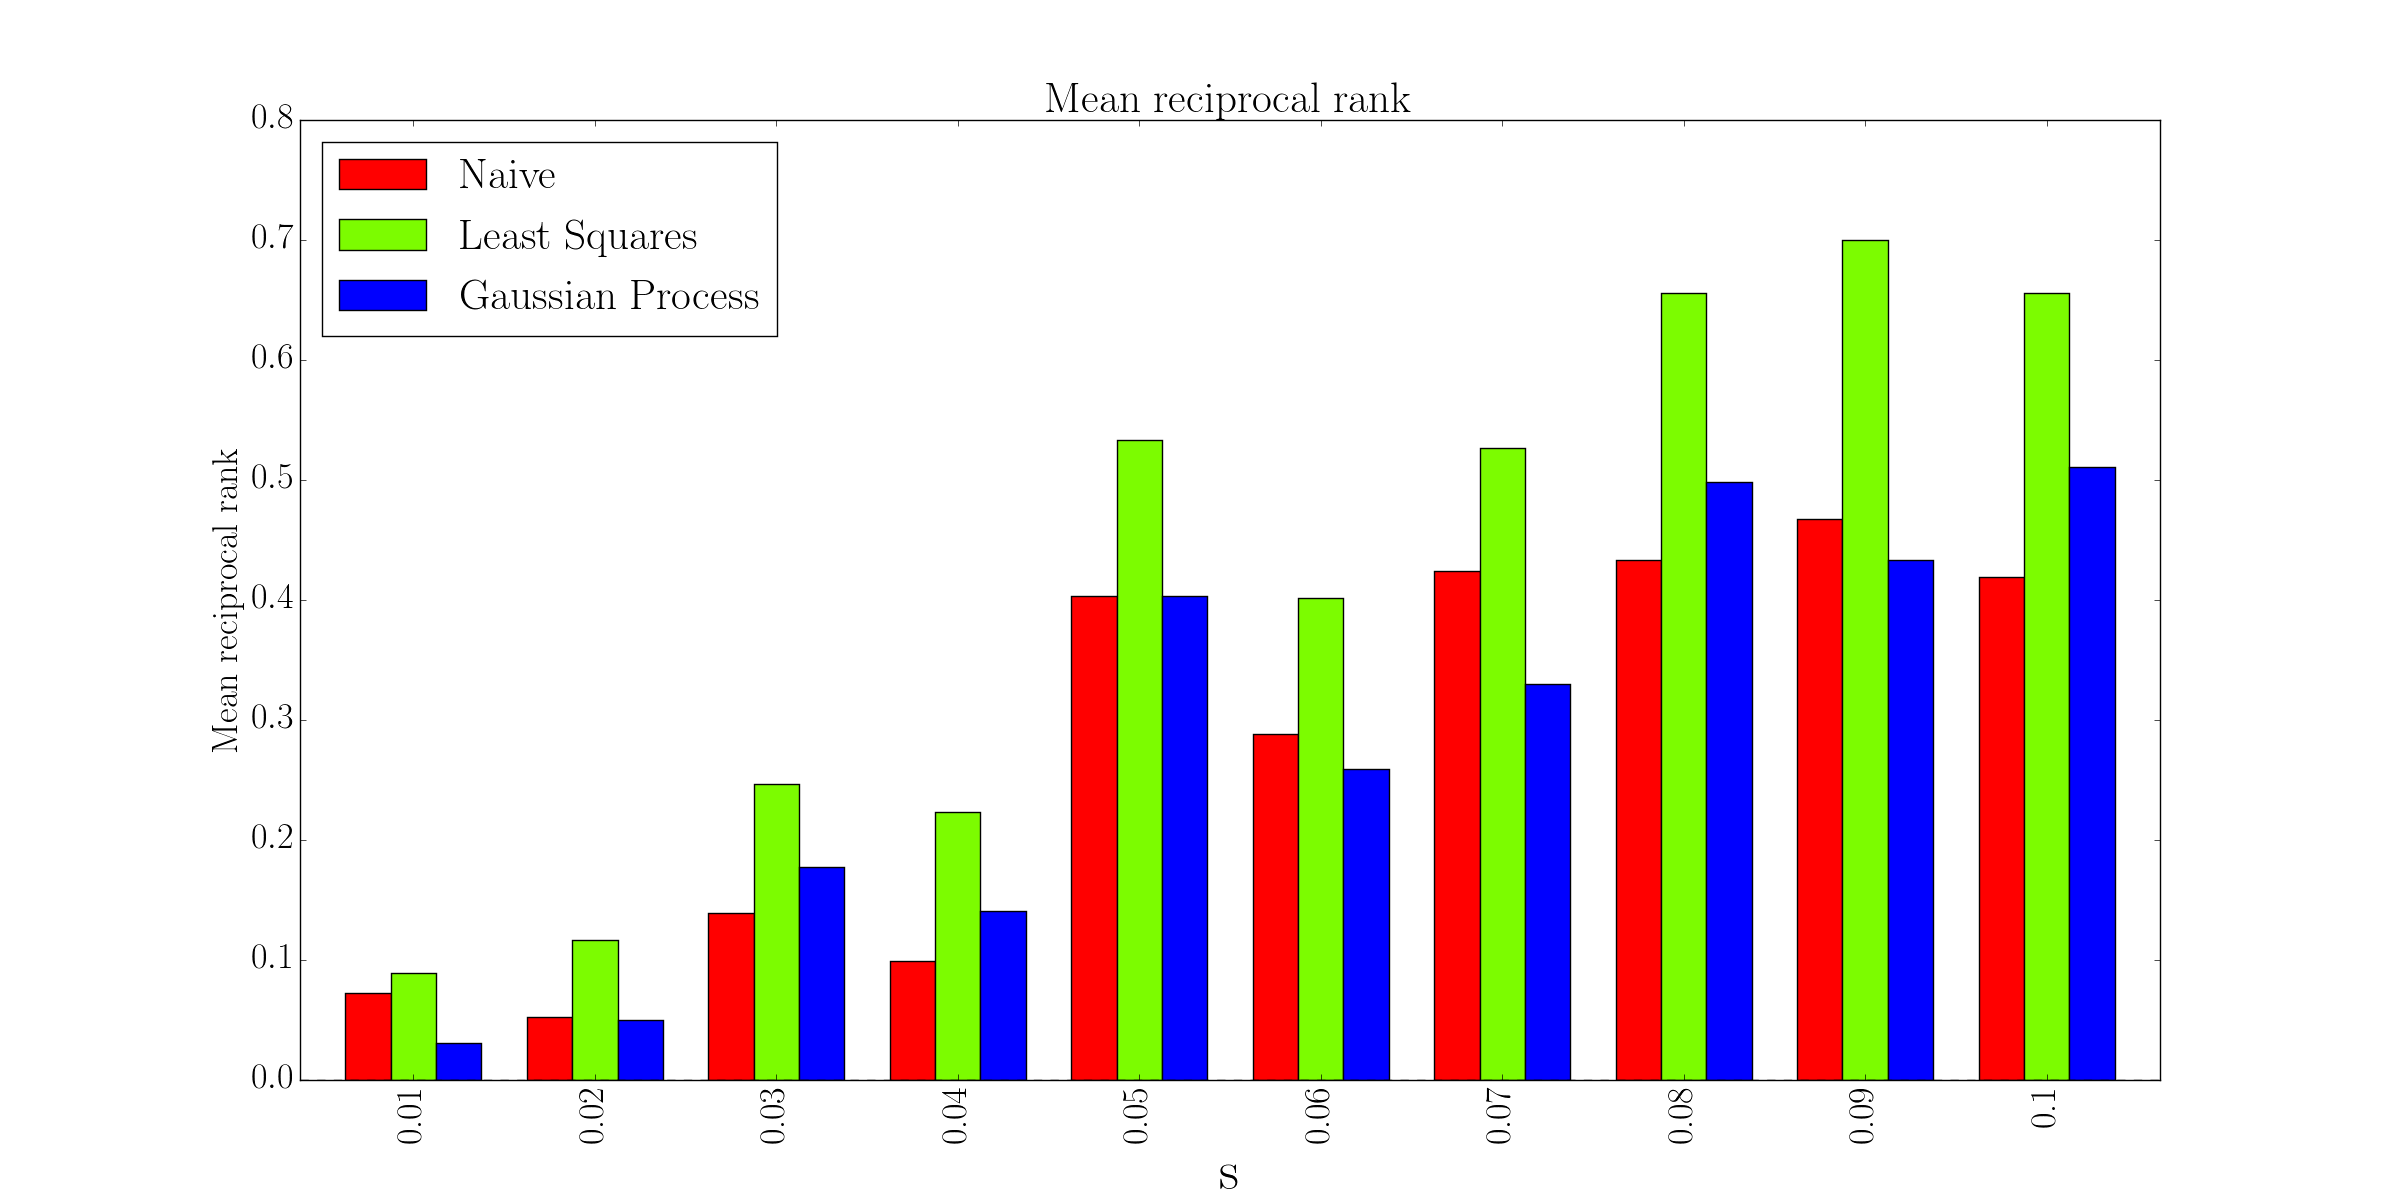
\includegraphics[width=\textwidth]{mrr}
  \caption{Mean Reciprocal}
  \label{fig:Fig2}
\end{figure}


\paragraph{Mean Average Precision (MAP)}
\begin{figure}[hh]
  \centering
    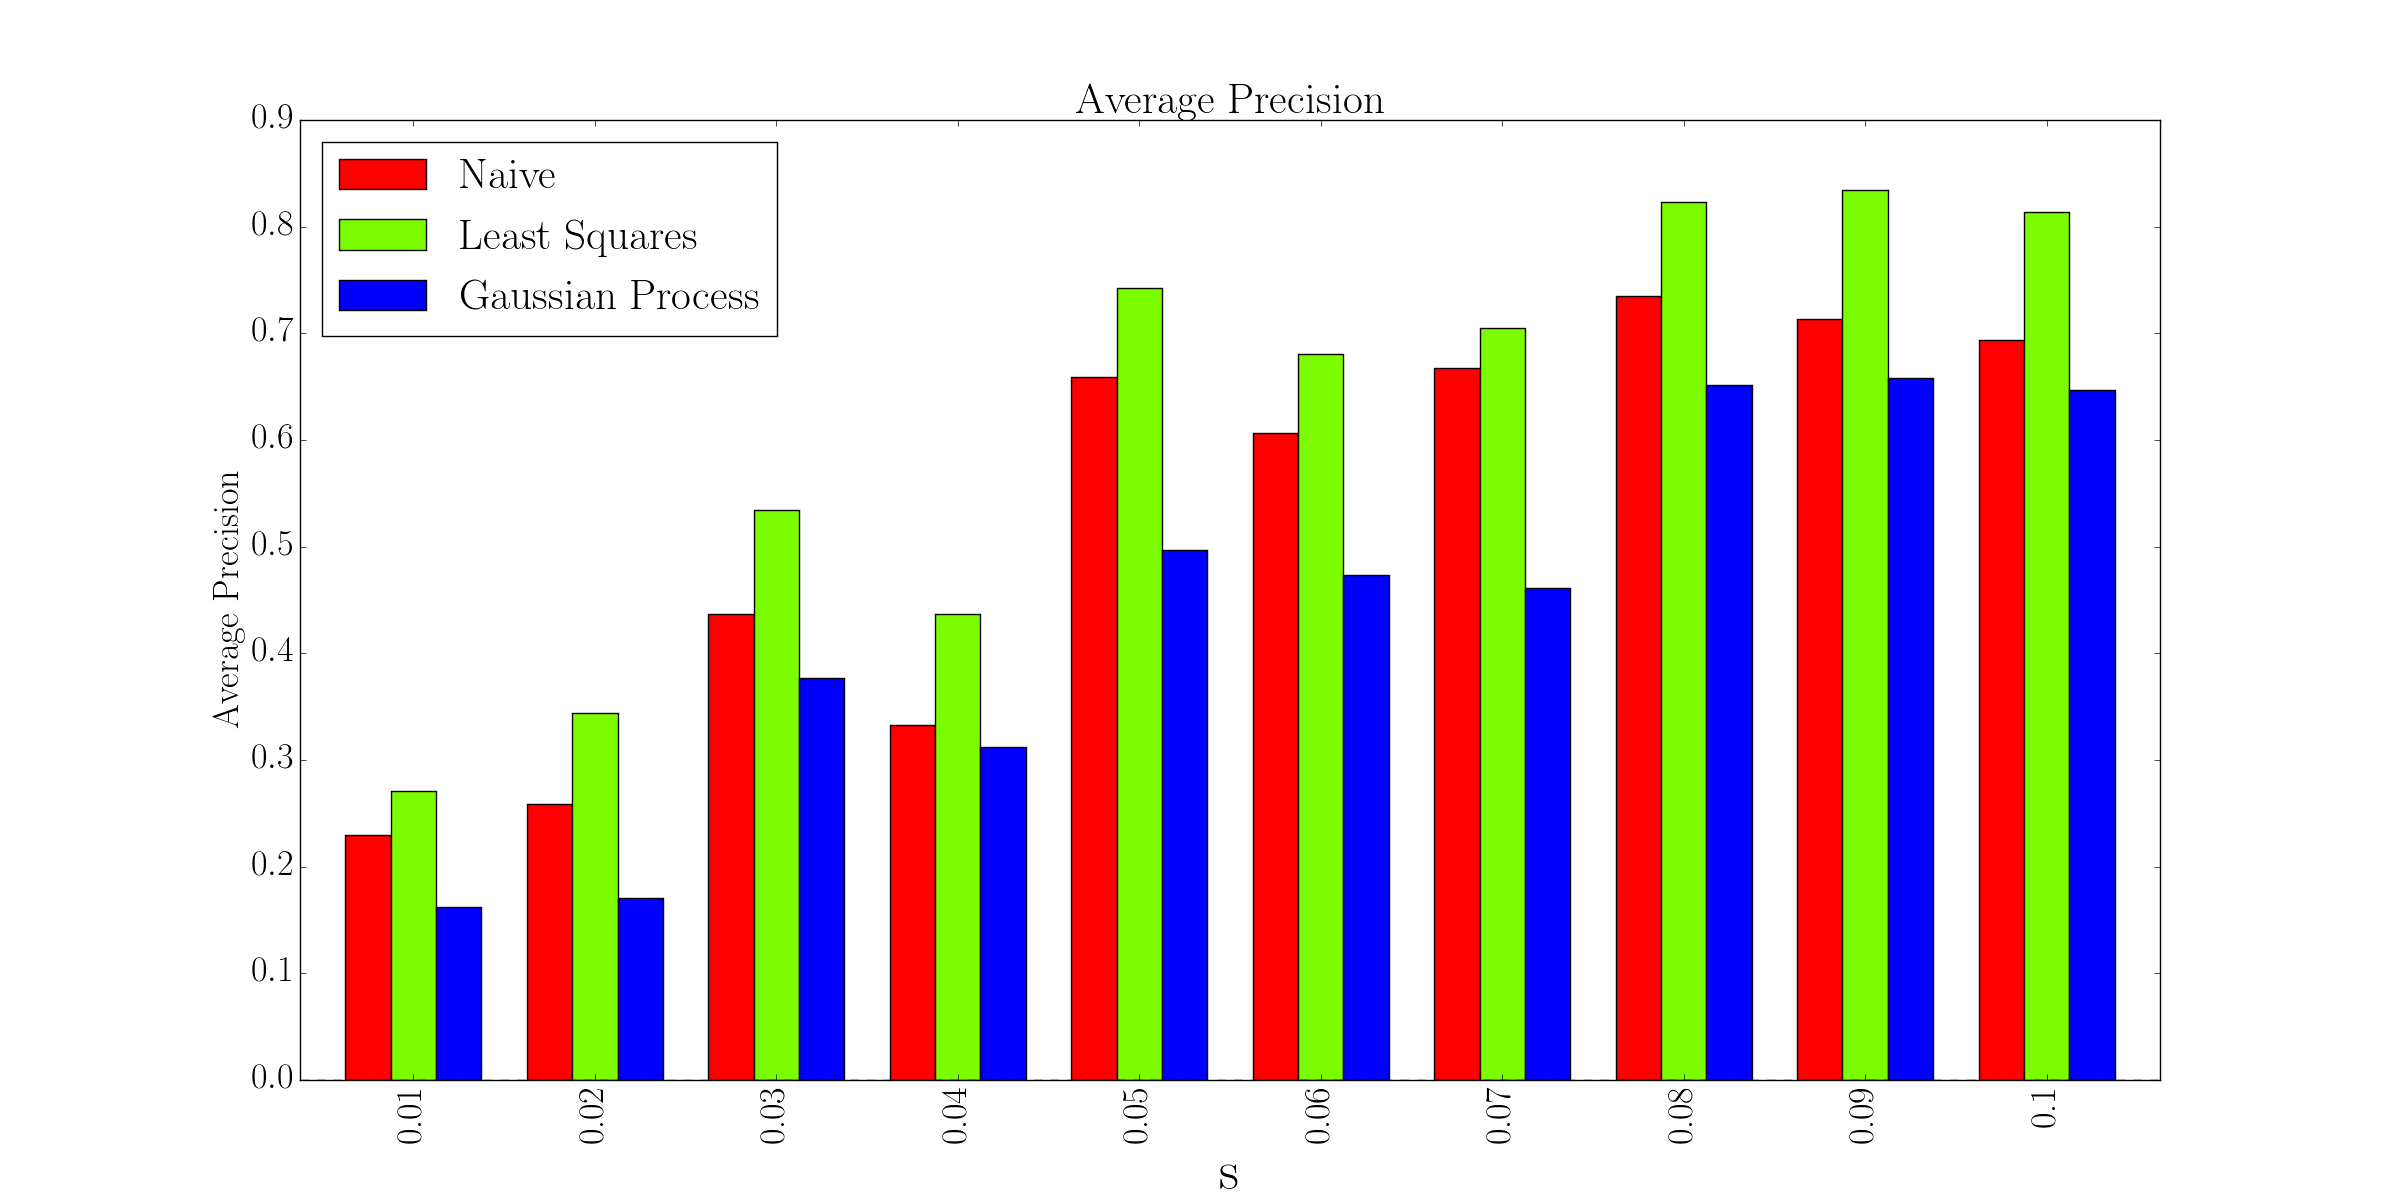
\includegraphics[width=\textwidth]{ap}
  \caption{Mean Average Precision (MAP)}
  \label{fig:Fig5}
\end{figure}


\subsubsection{Estimating Strength of Selection}
\begin{figure}[H]
  \centering
    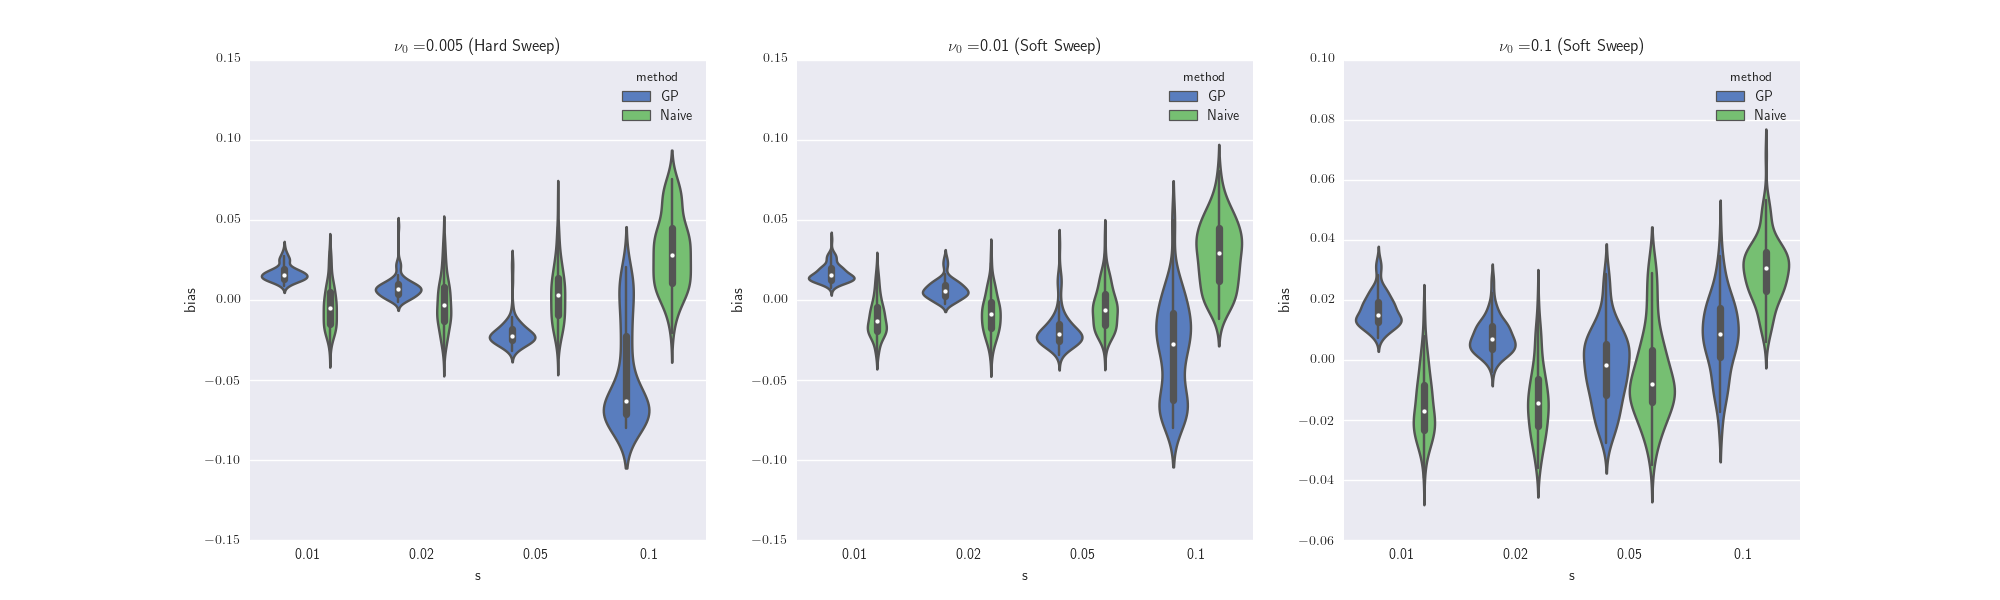
\includegraphics[width=\textwidth]{bias}
  \caption{Bias}
  \label{fig:Fig4}
\end{figure}

\subsection{Computational Performance}